\chapter{Simulation, data processing, and event reconstruction}\label{chap:reco}
The data sets, based on the proton-proton (pp) collisions recorded with the CMS detector, are centrally provided in the \texttt{MINIAOD} format~\cite{MiniAOD}. This format contains only parts of the original event and detector information relevant for most of the physics analyzes. An analysis looking for deviations from expectations from the SM is supposed not to be biased while development. Thus, SM and signal Monte-Carlo (MC) simulations are performed, and are centrally provided by the CMS collaboration. These are also provided in the \texttt{MINIAOD} format with extended generator information.\\
All available data sets, including measured data and simulation, are further processed with the help of the CMS software framework (CMSSW\footnote{Version 8.0.26})~\cite{CMSSW}, the CMS Remote Analysis Builder (CRAB3)~\cite{CRAB}, and the resources of the Worldwide LHC Computing Grid (WLCG)~\cite{Grid}, to obtain files with significantly reduced size. The obtained reduced information is stored in the \texttt{ROOT}~\cite{ROOT} file format, and can be used by analysts with self-developed software~\footnote{Usually composed of parts developed in \texttt{C/C++} and \texttt{Python}}.\\
\\
In this chapter, at first the used data samples are introduced. Thereafter, an overview of MC simulation is given, while the simulated samples used in this analysis are reviewed. After that, the event reconstruction performed on all data sets is explained. A more detailed view is given on the reconstruction and identification of physics objects.\\

Protons are very complicated objects composed of many different quarks and gluons. The probability to find a distinct parton of a proton in a deep-inelastic-scattering is given by Parton distribution functions (PDFs) and the underlying parton density functions~\cite{PDF}. Hence, an event measured with the CMS detector is not clean, but shows different effects. The interaction between the colliding two partons is described in the hard interaction. The products and quantities of these interactions contain the most interesting physical information. But, due to the structure of the proton, many different lower energetic particles can be produced in interactions between additional partons (multi-parton-interactions). These remnants of the scattering process, together with reconstructed remnants of the protons, are denoted as the underlying event. Interactions between protons in the same bunch crossing are referred to as pileup.

\section{Data sets}\label{sec:datasets}
This analysis uses different data sets based on the pp-collisions of the LHC with a center-of-mass energy of $13\TeV$ in 2016 and recorded with the CMS detector, corresponding to an integrated luminosity of $35.9\fbinv$. Each primary data set (PD) is a composition of events recorded with similar HLT trigger paths. The \texttt{DoubleMuon} and \texttt{DoubleEG} PDs are used in the central part of the analysis for the signal selection, since they contain events with two muons or electrons respectively. \texttt{MET} and \texttt{HT} PDs are used for trigger efficiency measurements, and the \texttt{MuonEG} PD is used to extract a selection relevant for the background prediction. For a list of used triggers see \refSec{sec:triggEff}.\\
The different PDs are separated into several single samples for different run eras throughout 2016. The paths of the used samples, available via the CMS data set bookkeeping service (DBS)~\cite{DASBookkeeping}, with the \texttt{03Feb2017} version of reconstruction are listed in \refTab{tab:datasets}.

\begin{table}[htb]
 \centering
 \caption{DBS paths for the datasets used in the analysis. Their path is similar, only the \texttt{PD} name varies. The dilepton data sets are used for the key analysis, whereas the $\HT$ and $\ptmiss$ datasets are used for the trigger efficiency measurement, see \refSec{sec:triggEff}.}
 \label{tab:datasets}
 \begin{tabular}{l|l}
  \hline
  \multirow{5}{*}{PDs}       & DoubleEG               \\
                             & DoubleMu               \\
                             & MuonEG                 \\
                             & HT                     \\
                             & MET                    \\\hline\hline
  \multirow{ 4}{*}{DBS path} & \verb|/PD/Run2016B-03Feb2017_ver2-v2/MINIAOD| \\
                             & \verb|/PD/Run2016(C-G)-03Feb2017-v1/MINIAOD| \\
                             & \verb|/PD/Run2016H-03Feb2017_ver2-v1/MINIAOD| \\
                             & \verb|/PD/Run2016H-03Feb2017_ver3-v1/MINIAOD| \\
  \hline
 \end{tabular}
\end{table}


\section{Simulation}\label{sec:Simulation}
The simulation process for SM background and SUSY signal samples can be divided in three major steps, which are very similar for both cases. At first, for a specific process events are simulated with an event generator. The event generators used for the generation of the samples considered in this analysis are \MADGRAPH5 in leading order (LO) configuration~\cite{Madgraph1,Madgraph2,Madgraph3}, \MADANDMC in next-to-leading order (NLO)~\cite{Madgraph1,AMCATNLO}, \PYTHIA~\cite{Pythia} for both cases of accuracy, or \POWHEG~\cite{Powheg1,Powheg2}. Matrix elements for the contributing diagrams are computed, and via convolving with PDFs, cross sections are calculated. These cross sections later can be used to rescale the MC simulation to a given integrated luminosity. Thus, the simulation can be performed with very high statistics and can still be compared to measured data.\\
Depending on the choice of the chosen generator, a separate generator for the simulation of hadronic showers must be used. This is done with \PYTHIA. Therewith partons generated in matrix element corresponding to the hard interaction, and partons generated with \PYTHIA in the showering for \eg initial state radiation (ISR), are not double counted, a matching with the \textsc{MLM}~\cite{Madgraph2} (LO) or \textsc{FXFX}~\cite{AMCATNLO} (NLO) matching schemes is performed. The hadronization of the partons (quarks and gluons) is simulated also with \PYTHIA, based on the confinement of color charged particles.  This, together with the underlying event and pileup, is all covered by the \textsc{CUETP8M1} generator tune~\cite{Tune}. It is based on $7\TeV$ proton-proton CMS and proton-antiproton CDF measurements. The PDFs used for the generation of the MC samples are provided by the \textsc{NNPDF} 3.0 sets~\cite{NNPDF}.\\
The big next step, which is the most time and resource consuming part, is the simulation of the detector response. A full model of the CMS detector was constructed with the \GEANTfour~\cite{Geant} package. Hence, it allows a precise simulation of the detector response for the events generated with the procedure described above. In the \GEANTfour package, material and particle properties, detector effects, and decay structures are considered in the simulation process. Since this procedure is very time consuming, but leads to a high accuracy, a different method is chosen for processes whose description is limited by different aspects. So for the generation of SUSY samples, where theoretical uncertainties dominate, the CMS \textsc{FASTSIM} packages is used~\cite{FastSim}. It is based on a simplified geometry and parametrizations, yielding a reduction in runtime of the factor $\approx100$. If the "FullSim" and "FastSim" performances are compared~\cite{FastSimQuality}, a agreement within $\approx10\%$ is observed.\\
\\
All MC simulated processes used in this analysis are listed in \refTab{tab:MCsamples} together with their corresponding cross sections used to rescale the samples later on. The DBS paths are given in the appendix in \refTab{tab:app_MCsets}.\\

\begin{table}[htb]
 \centering
 \caption{All SM model simulated samples used in the analysis with their cross sections. For their corresponding accuracy refer to the text. Additional k-factors to obtain NNLO cross sections for the $\PZ\PZ$ samples are applied per event in dependence of the $\pt$ of the diboson system. All samples are of the \texttt{MINIAODSIM} format.}
 % \scriptsize
 \label{tab:MCsamples}
 \begin{tabular}[width=\textwidth]{ll|ll}
  \hline
  \normalsize{process}                             & \normalsize{$\sigma\,[\mathrm{pb}]$} & \normalsize{process}                         & \normalsize{$\sigma\,[\mathrm{pb}]$} \\\hline
  \scriptsize{\textbf{ttbar}}                      &                                      & \scriptsize{\textbf{diboson}}                &                                      \\
  $\ttbar\to\ell^{+}\PGn\cPqb+\ell^{-}\PAGn\cPaqb$ & $87.31$                              & $\PZ\PGg\to2\ell\PGg$ ($\pt^{\PGg}<130\GeV$) & $124.936$                            \\
  \scriptsize{\textbf{ttbarGamma}}                 &                                      & $\PZ\PGg\to2\ell\PGg$ ($\pt^{\PGg}>130\GeV$) & $0.1488$                             \\
  $\ttbar\PGg\to2\ell2\PGn2\cPqb\PGg$              & $1.679$                              & $\PW\PZ$                                     & $4.9125$                             \\
  $\ttbar\PGg\to4\PQq2\cPqb\PGg$                   & $3.482$                              & $\PZ\PZ\to2\ell2\PGn$                        & $0.5644\cdot k(\pt^{ZZ})$            \\
  $\ttbar\PGg\to\ell\PGn2\cPqb2\PQq\PGg$           & $2.509$                              & $\PZ\PZ\to2\ell2\PGn$                        & $0.5644\cdot k(\pt^{ZZ})$            \\
  \scriptsize{\textbf{DrellYan}}                   &                                      & $\PW\PW\to2\ell2\PGn$                        & $12.178$                             \\
  $\PZ/\PGg^{*}\to2\ell$                           & $5765.4$                             & $\PW\Pg\to\ell\PGn\PGg$                      & $489$                                \\
  \textbf{single top}                              &                                      & \textbf{W jets}                              &                                      \\
  $\PWp\to\cPqt\cPaqb$                             & $3.36$                               & $\PW+jets$                                   & $61526.7$                            \\
  $\cPq\cPaqb\to\cPq^{'}\cPaqt$                    & $80.95$                              & \textbf{triboson}                            &                                      \\
  $\cPq\cPqb\to\cPq^{'}\cPqt$                      & $136.02$                             & $\PW\PW\PGg$                                 & $0.2147$                             \\
  $\cPaqb\to\PWp\cPaqt$                            & $11.7$                               & $\PW\PZ\PGg$                                 & $0.04123$                            \\
  $\cPqb\to\PWm\cPqt$                              & $11.7$                               &                                              &                                      \\
  \hline
 \end{tabular}
\end{table}



The Drell-Yan (DY) $\PZ/\PGg$ process, as well as the diboson $\PZ\PGg$ and $\PW\PGg$ processes, and triboson production of $\PW\PW\PGg$ and $\PW\PZ\PGg$ are generated with \MADANDMC in NLO. Top pair production in association with a photon ($\ttbar\PGg$) and the production of a $\PW$ boson in association with jets are also simulated using the \MADANDMC generator in NLO. Top pair production with leptonic decays ($\ttbar\to 2\ell 2\PGn 2\cPqb$), diboson production of $\PW\PZ$, $\PZ\PZ$, $\PW\PW$, and all singletop production processes are generated using \POWHEG.
The diboson $\PW\PW$ and $\PW\PGg$ production, the production of $\PW+jets$, triboson $\PW\PW\PGg$ and $\PW\PZ\PGg$ production, and all singletop production channels are grouped together and denoted as "other" in the following.
Next-to-leading order and next-to-next-to-leading order (NNLO) cross sections~\cite{xsec1,xsec2,xsec3,xsec4,xsec5,xsec6,xsec7,xsec8,xsec9} are used for the normalization of the samples.\\
The generator used for the signal simulation production is \MADGRAPH\_\MCATNLO for the simplified models, and \PYTHIA8 for the full GGM model. The corresponding DBS paths are also listed in the appendix in \refTab{tab:app_signalsets}.
The cross sections used in the signal normalization are calculated at NLO accuracy for the full GGM scenario, and at NLO+next-to-leading logarithmic (NLL) accuracy for the two simplified models~\cite{sxsec1,sxsec2,sxsec3,sxsec4,sxsec5,sxsec6,sxsec7,sxsec8,sxsec9}.
For the electroweak SMS, the applied cross section is calculated for $\charginoOne\neutralinoOne$ and $\charginoOne\charginoOneBar$ production with squarks and gluinos decoupled, and the sum of both is used. In the cross section calculation of gluino pair production for the other SMS, squark decoupling is assumed. The applied cross sections for the GGM scenario are obtained using a full model, thus being different from the ones used for the electroweak SMS.\\
For the GGM model signal points are generated with wino masses ranging from $215\GeV$ to $1015\GeV$, and bino masses from $205\GeV$ to $m(\widetilde{W})-10\GeV$ in intervals of $25\GeV$.
In case of the \texttt{TChiZG} SMS, points are generated with NLSP masses in the range of $300-1300\GeV$ in steps of $25\GeV$. The grid of points generated for the \texttt{T5bbbbZG} strong production SMS includes gluino masses in the range of $800\GeV$ to $2500\GeV$, while the NLSP mass range is scanned from $10\GeV$ to $m(\widetilde{g})-10\GeV$ in non equidistant steps.\\
\\
As mentioned above, the true number of generated MC events $N_{Gen}$ is very high. Thus, together with the measured integrated luminosity $\Lumi$, and a given cross section $\sigma$, a global event weight of
\begin{equation}
 w = \frac{\Lumi \cdot \sigma}{N_{Gen}}
\end{equation}
is obtained.\\
Additional event weights are applied on the simulation to account for differences in the pile up distribution. To improve on the \MADGRAPH modeling of the multiplicity of additional jets arising from initial state radiation, SUSY SMS MC events are reweighted as a function of $N^{ISR}_{Jet}$ or the transverse momentum of the ISR system, to improve the agreement with observations in data.
The latter is based on studies of the transverse momentum of $\PZ$ events.~\cite{NISRweight}.
The differences to 1 for the reweighting factor is considered as a systematic uncertainty later on.
The \POWHEG \ttbar simulation is also reweighted as a function of the transverse momentum of the top system, based on studies in top pair production cross section measurements~\cite{topWeight1,topWeight2,topWeight3,topWeight4} to improve the agreement of the transverse momentum of the top quark with data.

\subsection*{Overlap Removal}\section{sec:overlap}

Because different samples are used in the case of top pair production and Drell-Yan for the nominal process and additional photon production in the hard interaction, there exists an overlap between those simulated samples. This is the case, since the photon production in the hard interaction is physically the same as photon radiation in the initial state. Hence, this overlap needs to be removed. Therefore, events that show a signature like the one simulated in the exclusive hard photon interaction samples, are removed on generator level from the nominal MC samples. So after applying the procedure ,both samples can be added, and double counting of diagram contributions is rejected.

\section{Event and particle reconstruction and identification}\label{sec:reco}
To maintain both, a precise and robust particle reconstruction, and flexibility in the physical object identification, particle reconstruction and identification is divided in two major parts. At first, particles and their properties, such as momentum, energy, and trajectory, are reconstructed with the Particle Flow (PF) algorithm~\cite{ParticleFlow} by combining information from all CMS subdetectors. After that, identification criteria determined by specialized CMS physics objects groups (POGs) are applied, dependent on the choice of the analyst regarding efficiency and misidentification rates.\\
In the following the PF algorithm is briefly introduced by explaining its main features, and more detailed definitions of the physical objects are given.

\subsection{Particle Flow}
Particles are reconstructed and categorized by PF in five classes, namely muons, electrons, photons, and both neutral and charged hadrons. The decisions are made based on two major reconstruction steps, finding and reconstructing tracks of charged particles, and separate clustering of ECAL and HCAL entries, to reconstruct the energy deposit of the particles' showers.\\
The track finding algorithm based on Kalman filtering~\cite{Kalman} iteratively generates seeds for the tracks, builds trajectories, and performs a final fit to determine the particle properties, such as direction and momentum based on information of the inner tracker.
For particles such as muons and electrons, additional tracking algorithms are used to determine a more accurate description of the particle's properties. For muons, additional information of the muon system is used to directly classify three types of non exclusive muon tracks. Standalone muon tracks are reconstructed using only informations of the muon system. If inner tracker tracks can be matched to entries in the muon system, they are called tracker muon track. And in cases where muon system tracks are matched to inner tracks, these are called global muon tracks.
For electrons additional fitting procedures combining tracker and ECAL informations are used to cope the characteristics of the electromagnetic showers~\cite{GSFTrack}. Therefore, superclusters are built within the ECAL by combining nearby clusters, and the seeds determined with the tracker based approach described above, together with this ECAL based reconstructed seeds, are used in a common track fit.\\
The clustering algorithm for the ECAL and HCAL also determines cluster seeds at first based on local energy maxima, and afterwards adds cluster entries fulfilling certain energy criteria to obtain topological clusters.\\
The following combination and linking of the determined information is motivated by the main characteristics of the particle interactions:\\
Photons are neutral particles, and therefore leave no track in the detector, but only interact electromagnetic. Thus, they are stopped in the ECAL by generating electromagnetic showers. They can also undergo electron-positron pair production, resulting also in electromagnetic showers in the ECAL.\\
Electrons are charged particles. Hence, their tracks are reconstructable in the tracker, and the energy deposit happens also via electromagnetic shower generation due to Bremsstrahlung in the ECAL. Accordingly, electrons and photons are very similar objects in the reconstruction procedure.\\
Muons are mainly identified by the informations of the muon system, since no other particles except for very high energetic jets punching through the solenoid and outer HCAL, are capable of reaching the muon chambers. By combining the inner tracks with the entries of the muon chambers, a clear and precise muon identification is maintained.\\
Charged and neutral hadrons are reconstructed by clusters in the HCAL, and can be differentiated by corresponding matching tracks in the tracker. Parts of non-prompt photons, \eg coming from meson decays, are also reconstructed as neutral hadrons.\\
The order of particle reconstruction is based on the accuracy and precision of the available information. Thus, muons are identified first, followed by electrons and prompt photons. After that, neutral and charged hadrons, and non-prompt photons are identified.\\
All these informations obtained by the PF algorithm provide the basis for the final physical object identification applied by the analysts.

\subsection{Primary vertex}
The primary vertex is defined by the vertex with the largest sum of transverse momenta determined by vertex reconstruction algorithms~\cite{vertex}, and needs to be reconstructed within a distance of $24\cm$ in z direction, and $2\cm$ in the x-y-plane.


\subsection{Muons}
Muons are required to have a transverse momentum larger than $15\GeV$. And because the muon chambers extend only to a pseudorapidity range of $|\eta|<2.4$, muons need to be reconstructed within this region. In addition, muons have to pass a some quality requirements obtained by the muon POG, yielding a $\approx 98\%$ efficiency~\cite{MuonIDPerf}.\\
The muon needs to be reconstructed as a PF muon, and either as a global muon or a tracker muon. If it is reconstructed as a global and a tracker muon, the segment compatibility, which is a measure for the comparability between the tracker tracks and an extrapolation to the muon system, has to be larger than $0.303$. In addition, more than $80\%$ of the inner track layers need to be used within the track fit, the normalized goodness of fit ($\chi^2/ndof$) needs to be less than $3$, the match between the standalone muon position and the tracker muon must have $\chi^2<12$, and the maximum $\chi^2$ found by a kink finding algorithm, which tries to separate the track into two independent tracks, needs to be smaller than $20$. If the muon is reconstructed exclusively as a tracker muon, only the segment compatibility needs to be greater than $0.451$, and the other requirements on the track quality are removed.\\
Besides the identification requirements, conditions on the position of the track relative to the reconstructed primary vertex are imposed. In the transversal direction ($d_{xy}$), muon tracks need to be closer than $0.05\cm$ to the vertex, and in the longitudinal direction ($d_z$), the distance needs to be smaller than $0.1\cm$. A cone dependent isolation is introduced, called "mini isolation", where the cone size in the $\phi-\eta$ plane is calculated relative to the transverse momentum of the particle as follows:
\begin{equation}
 R = max\left(0.05,min\left(0.2,\frac{10\GeV}{\pt}\right)\right).
\end{equation}
Pile up corrections are also taken into account in the mini isolation calculation.
The determined energy deposit in the cone around the muon must not exceed $10\%$ of the transverse momentum of the particle.


% \begin{table}[h!]
%  \label{tab:muonID}
%  \centering
%  \begin{tabular}{ll}
%   variable                                            & requirement \\\hline
%   global muon                                         & true        \\
%   fraction of valid inner tracker hits                & $>0.8$      \\
%   normalized $\chi^2$ of global track                 & $<3$        \\
%   chi2localposition (track standalone position match) & $<12$       \\
%   kink finder                                         & $<20$       \\
%   segment compability                                 & $>0.451$
%  \end{tabular}
% \end{table}



\subsection{Electrons}
The list of requirements imposed on the electron selection is driven by a symmetric approach between the two lepton selections. The same conditions on the distance to the primary vertex, ($d_{xy}<0.05$, $d_z<0.1$), the maximum pseudorapidity ($|\eta|<2.4$), and transverse momentum ($\pt>15\GeV$) need to be fulfilled. The mini isolation criterion is relaxed to $20\%$.\\
The identification requirements determined by the EGamma POG~\cite{ElectronID} separately for electrons reconstructed in the ECAL barrel (EB: $|\eta_{Supercluster}|<1.479$) and endcap (EE: $|\eta_{Supercluster}|>1.479$) region are listed in \refTab{tab:eleID}.
\begin{table}[h!]
 \centering
 \caption{Identification criteria for electrons given separately for reconstructed electrons in the barrel and endcap.}
 \label{tab:eleID}
 \begin{tabular}{lcc}
  Variable                       & \multicolumn{2}{c}{Value}              \\\hline
                                 & EB                        & EE         \\\hline
  $\sigma_{i\eta i\eta}$         & $<0.00988$                & $<0.0298$  \\
  $\Delta\eta_{Seed}$            & $<0.00311$                & $<0.00609$ \\
  $\Delta\phi_{In}$              & $<0.00311$                & $<0.00609$ \\
  $H/E$                          & $<0.253$                  & $0.0878$   \\
  relative combined PF isolation & $<0.0695$                 & $<0.0821$  \\
  $|\frac{1}{E}-\frac{1}{p}|$    & $<0.134$                  & $<0.13$    \\
  \# missing inner hits          & $\leq1$                   & $\leq1$    \\
  Photon conversion veto         & true                      & true       \\\hline
 \end{tabular}
\end{table}
Here, $\sigma_{i\eta i\eta}$ is a quantity characterizing the width of the electromagnetic shower shape in the ECAL in the $\eta$ direction. It is calculated as a weighted variance of energy deposits in the full 5x5 pixel ECAL supercluster. Since jets emerging from hadrons have a wider shower in the ECAL than electrons, a differentiation can be achieved. Consistency between the information of the reconstructed track at the vertex, and the supercluster is required, by setting conditions on $\Delta\eta$, $\Delta\phi$, and the supercluster energy $E$ and track momentum $p$. To further separate electrons from hadrons, more energy should be deposited in the ECAL, rather than in the HCAL ($H/E$). An isolation requirement based on the PF determined isolation, assures that prompt electrons are separated from electrons coming from \eg jets. Contributions from photons faking electron signatures are suppressed by imposing a requirement on the number of missing inner hits in the tracker, and an additional veto for photon conversions to electron-positron pairs determined in an $\chi^2$ fit.

\subsection{Photons}
Photons need to have a transverse momentum larger than $20\GeV$. Because photons are produced more centrally due to the high masses and short lifetimes in the considered SUSY signal scenarios, only photons reconstructed in the ECAL barrel are considered ($|\eta<1.4442|$). Additional identification criteria determined by the EGamma POG~\cite{photonID} are listed in \refTab{tab:photonID}.
\begin{table}[h!]
 \centering
 \caption{Identification criteria for photons reconstructed in the ECAL barrel.}
 \label{tab:photonID}
 \begin{tabular}{lc}
  Variable                    & Value                                                \\\hline
  $\sigma_{i\eta i\eta}$      & $<0.01031$                                           \\
  $H/E$                       & $<0.0597$                                            \\
  PF charged hadron isolation & $<1.295$                                             \\
  PF neutral hadron isolation & $<10.910 + 0.0148 \cdot \pt + 0.000017\cdot (\pt)^2$ \\
  PF photon isolation         & $<3.630+0.0047\cdot \pt$                             \\\hline
 \end{tabular}
\end{table}
Similar to the requirements on $\sigma_{i\eta i\eta}$ and $H/E$ for the electron selection, these conditions in the photon identification ensure the suppression of selecting hadrons faking the photon signature. Additional different isolation criteria lower the amount of selected photons originating from neutral and charged hadrons, and photons coming from light meson decays.\\
Requirements on the distance in the $\eta-\phi$ plane between the photon and selected lepton candidates ($\Delta R(\PGg,\ell)>0.3$) significantly reduce contributions from final state radiation (FSR) photons. By requiring that no pixel seed can be assigned to a trajectory between ECAL supercluster and interaction point, a clear differentiation between electrons and photons is achieved.

\subsection{Jets}
Jets, see \refSec{sec:SM}, are very complicated objects due to the complexity of the hadronization and fragmentation processes. Therefore, a sophisticated clustering algorithm is needed to measure the energy of jets properly. Jets are clustered with the anti-$k_T$ algorithm~\cite{AntiKT} included in the \FASTJET package~\cite{FastJet1,FastJet2} with a distance parameter of $R=0.4$. The jet momentum is defined as the total sum of the momenta of the constituents of the jet. Charged hadrons not emerging from the primary vertex are not considered in the clustering. The jet energy is corrected for effects originating from pile up and the detector response, tuned with the help of different data control selections and simulation~\cite{JEC}. Reconstructed jets need to pass a loose ID proposed by the Jet-Missing Transverse Energy POG~\cite{JetID}, need to have a transverse momentum larger than $30\GeV$, and the pseudorapidity must not exceed $|\eta|=3,$. In addition, jets overlapping with photon and lepton candidates in a cone with radius $R=0.4$ in the $\eta-\phi$-plane, are removed from the selection to forbid double counting of objects.

\subsection{Missing transverse momentum}
The missing transverse momentum $\ptmiss$ is one of the most important observables in searches for BSM physics. In typical SUSY models, see \refSec{sec:SUSY}, a significant amount of $\ptmiss$ is expected in the events due to the LSP. In SM processes only neutrinos and mismeasurements of \eg the jet energies lead to missing transverse momentum, because before a collision the transverse momentum of the colliding protons is nearly negligible. Hence, the missing transverse momentum quantifies the imbalance of all reconstructed particles in an event and is defined as
\begin{equation}
 \ptmiss= |\ptvecmiss| = |-\sum_{PF objects}\pt_{,i}|.
\end{equation}
Jet energy corrections are propagated to the missing transverse momentum vector to reduce a strong bias in events with large hadronic activity.

\section{Definition of observables}
Throughout this thesis different observables are used to define different phasespace regions, in particular the signal region and control and validation regions important for the background prediction. All these high level variables are defined based on low level quantities such as the $\pt$ of different objects, or are calculated by complex algorithms combining them.

\subsection*{Total hadronic activity $\HT$}
The hadronic activity $\HT$ is defined as the scalar sum of all jets transverse momenta
\begin{equation}
 \HT = \sum_{Jets} |\ptvec_i|.
\end{equation}

\subsection*{The transverse mass $m_{T}$}
The transverse mass of two objects with transverse momentum $\ptvec^A$ and $\ptvec^B$ yields the transverse mass of the mother particle if both particle emerge from the same decay. In cases of invisible decay products, the transverse mass is an estimate of the mother mass in the transverse plane. Therefore it is a good estimate for the total mother particle mass, because the missing momentum can only be determined in the transverse plane. It is defined as
\begin{equation}
 m_T\left(\ptvec^{A},\ptvec^B\right) = \sqrt{2|\ptvec^A||\ptvec^B|\left(1-\cos(\Delta\phi)\right)},
\end{equation}
where $\Delta\phi$ is the angle between $\ptvec^A$ and $\ptvec^B$ in the transverse plane.

\subsection*{The stransverse mass $\mtTwo$}
In case of two identical particles, decaying both to one invisible and one visible particle, the stransverse mass $\mtTwo$~\cite{Mt2_1,Mt2_2} is a useful generalization of $m_T$. In this analysis it is calculated to estimate the mass of the NLSP, which decays to an invisible object, the gravitino, and one visible particle, a Z boson or a photon. It is defined as
\begin{equation}
 \mtTwo = min_{\ptvec^{\Pgn_1}+\ptvec^{\Pgn_2}=\ptvecmiss}\left(max\left[m_T(\ptvec^{\PZ},\ptvec^{\Pgn_1}),m_T(\ptvec^{\PGg},\ptvec^{\PGn_2})\right]\right),
\end{equation}
where the final value is determined via minimization as indicated by $min$ in the equation. Descriptively, the algorithm tries to estimate the transverse mass of the mother particle under the assumption, that the $\ptmiss$ is composited of exactly two identical particles each from one decay branch.\\
For decays of the NLSP in all signal models, the $\mtTwo$ distribution has a cut-off at the mass of the lightest neutralino, while for all SM backgrounds $\mtTwo$ yields much lower values in comparison to the high SUSY masses. See \refFig{fig:mt2} for a visualization.

\begin{figure}
 \centering
 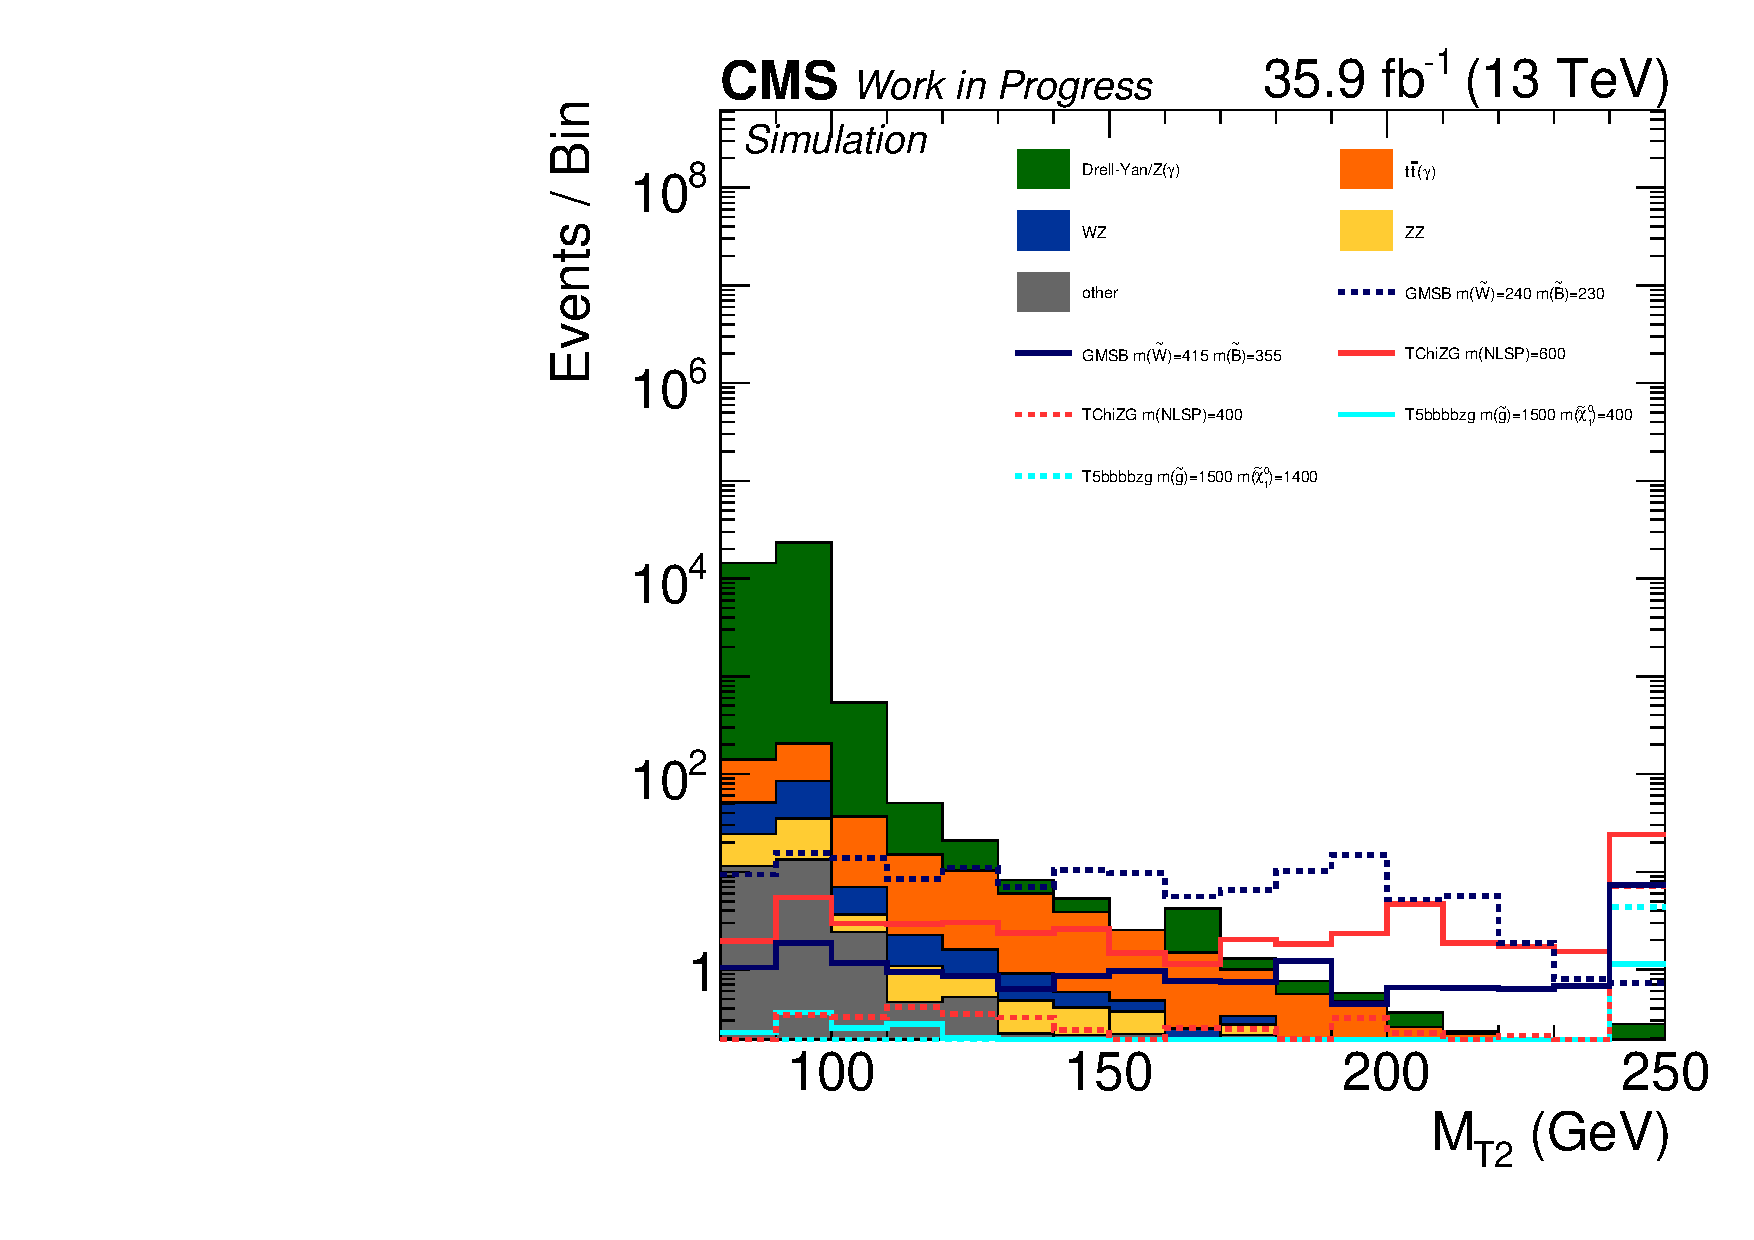
\includegraphics[width=\pairwidth]{figures/mt2/onZ_LL_mt2_log}
 \caption{Stacked background and different signal points against the stransverse mass $\mtTwo$. Both are obtained from simulation. For each signal model two different signal points are shown. For their masses refer to the legend in the plot.}
 \label{fig:mt2}
\end{figure}


\section{Lepton pair selection and quality requirements}\label{sec:lepPair}
In the analysis, different datasets triggered with different dilepton triggers are combined, see \refSec{sec:datasets}. Therefore it is possible, that an event is contained in more than one data set. Hence, it is assured with the following procedure, that no event is double counted. At first, all leptons per event are sorted by their transverse momenta. Thus, the leading and subleading lepton\footnote{It is called trailing from now on.}, are identified. Their flavor combination then determines the classification of the event as "dielectron", "dimuon", or "electron-muon". For instance, an dielectron event is classified as such, if there are at least two electrons in the event, the event originates from the \texttt{DoubleEG} sample, both the leading and the trailing lepton are electrons, and it is triggered by at least one of the dielectron triggers. This set of conditions ensures the exclusivity of the three selections.\\
In addition, there are some requirements imposed on the dilepton system. The trailing and leading lepton need to be separated at least by a distance of $\Delta R=0.1$ in the transverse plane, and the invariant dilepton mass $m_{\ell\ell}$ should be larger than $50\GeV$. The first requirement provides a cleaning between the lepton collections and ensures, that no lepton is counted twice, while the latter threshold is introduced, because the simulation of the Drell-Yan simulation does not include events with lower dilepton masses~\footnote{Events with lower invariant dilepton masses are not of interest for this analysis, since in the following only leptons originating from a Z boson decay are selected, resulting in an invariant dilepton mass around the Z boson mass of $\approx91\GeV$.}.\\
Hereafter, the dielectron and dimuon selections are combined to a dilepton selection to increase the statistics in the validation, and especially in the signal region.\\
Additional leptons need to pass the same selection of the trailing lepton.
\\
Also, several event quality filters are applied to reject contaminated events. The list of applied filters is recommended by the POGs~\cite{MetFilter}. It reads:
\begin{itemize}
 \item \texttt{HBHE noise filter}
 \item \texttt{HBHE noise iso filter}
 \item \texttt{ECAL TP filter}
 \item \texttt{eeBadSCFilter}
 \item \texttt{bad PF muon filter}
 \item \texttt{bad charged hadron filter}
 \item \texttt{bad muon filter}
 \item \texttt{beam halo filter}
\end{itemize}
The rejected events consist mainly of events with faulty detector signals, cosmic muons, or muons produced in scattering processes with the beam halo.


\section{Used triggers and trigger efficiency measurement}\label{sec:triggEff}
\todo{Erwaehnen, dass leading leg auch gemessen wird. Vll plot zeigen. Siehe marcs frage.}
As already pointed out in \refSec{sec:datasets}, the events are recorded with various dilepton triggers. For each dilepton combination ($\Pe\Pe,\Pgm\Pgm,\Pe\Pgm$) multiple triggers are used because of the changing instantaneous luminosity over the 2016 run period, and different triggers were active at different times. The main trigger paths are isolated dilepton triggers, while non-isolated trigger paths are added to increase the efficiency for boosted topologies of the dilepton system. A list of all used HLT trigger paths is given in the appendix in \refTab{tab:app_trigger}. While the same flavor dilepton triggers ($\Pe\Pe,\Pgm\Pgm$) are used as signal triggers, the different flavor triggers ($\Pe\Pgm$) are used to select events needed for the background prediction of the top pair production ($\ttbar(\PGg)$) background. This will be explained in more in detail in \refSec{sec:ttbar}. The dilepton triggers alltogether have transverse momentum thresholds for the dileptons of around $17-33\GeV$ for the leading lepton, and $8-33\GeV$ for the trailing one. Additional triggers with hadronic activity ($\HT$) or $\ptmiss$ thresholds are relevant for the trigger efficiency measurement, which will be presented in the following.
\subsection{Trigger efficiency measurement}
A trigger efficiency curve is characterized by an inefficient part, a more or less sharp transition ("Turn On") to the efficient part ideally located at the nominal threshold of the trigger path, and a flat efficient part called plateau.\\
Hence, measuring the trigger efficiency is essential to obtain appropriate transverse momentum requirements for the dilepton system. Furthermore, in the signal MC simulation using the \textsc{FASTSIM} package no trigger simulation is performed, like it is done for the SM background samples. Therefore, the efficiency needs to be measured also on simulation, such that the signal simulation can be scaled accordingly. In addition, the SM simulation samples will be weighted with a further factor, correcting for differences in the efficiency between data and simulation.\\
As indicated, not a single signal trigger or a single trigger for the control region selection is used, but a logical \texttt{OR} combination of all dilepton triggers with the same flavor requirements is used. Thus, for an event only one of the used triggers has to be fired to be selected for the key analysis. Because the total number of produced events including triggered and non triggered events in CMS is not available apparently for data\footnote{For simulation these informations are available. This is used for further checks to validate the procedure of efficiency measurement.}, the combined trigger efficiency $\varepsilon$ is measured using a baseline trigger. Thus, it is defined as the number of events passing baseline and signal trigger, divided be the number of events passing only the baseline trigger:
\begin{equation}
 \varepsilon=\frac{\#(baseline \wedge signal)}{baseline}.
\end{equation}
As a consequence, the contribution of the baseline trigger cancels, and the pure signal trigger efficiency is maintained. As baseline triggers a combination of various triggers with $\HT$ thresholds is used. These thresholds range from $200-800\GeV$. Therefore, the measurement is not performed on the dilepton data streams, but on the $\HT$ datasets. The event selection consists basically of the lepton pair selection introduced in \refSec{sec:lepPair} with an additional $\HT>200\GeV$ requirement to ensure, that the baseline triggers are fully efficient. An additional matching between the selected leptons and the trigger objects responsible for the firing of the trigger is performed. Resulting efficiency curves for all three dilepton combinations measured both on data and simulation are shown in \refFig{fig:triggEff} against the $\pt$ of the trailing lepton. The statistical uncertainties of the individual bins are calculated using $95\%$ confidence level (CL) Clopper-Pearson intervals~\cite{ClopperPearson}. The measurements suffer mainly from statistics on data, while the statistics of the simulation is very high per definition. The electron-muon channel is affected the most by this effect. However, the efficiency curves show the structure of multiple Turn Ons, as it is expected from a combination of triggers with very different ranges of thresholds. As indicated by the dotted lines in the plots, the lepton $\pt$ cut was determined to be $20\GeV$ for the trailing lepton, and $25\GeV$ for the leading one. Although the dielectron and electron-muon triggers are not yet that fully efficient at this threshold as it is the case for the dimuon trigger, this requirement is imposed also on the other to selections in order to obtain a symmetric lepton selection. The mean plateau efficiencies are shown as a gray band with its statistical uncertainty in the plots. The mean efficiency is also measured on simulation, and all values are given in \refTab{tab:triggEff}.
\begin{figure}[htb]
 \centering
 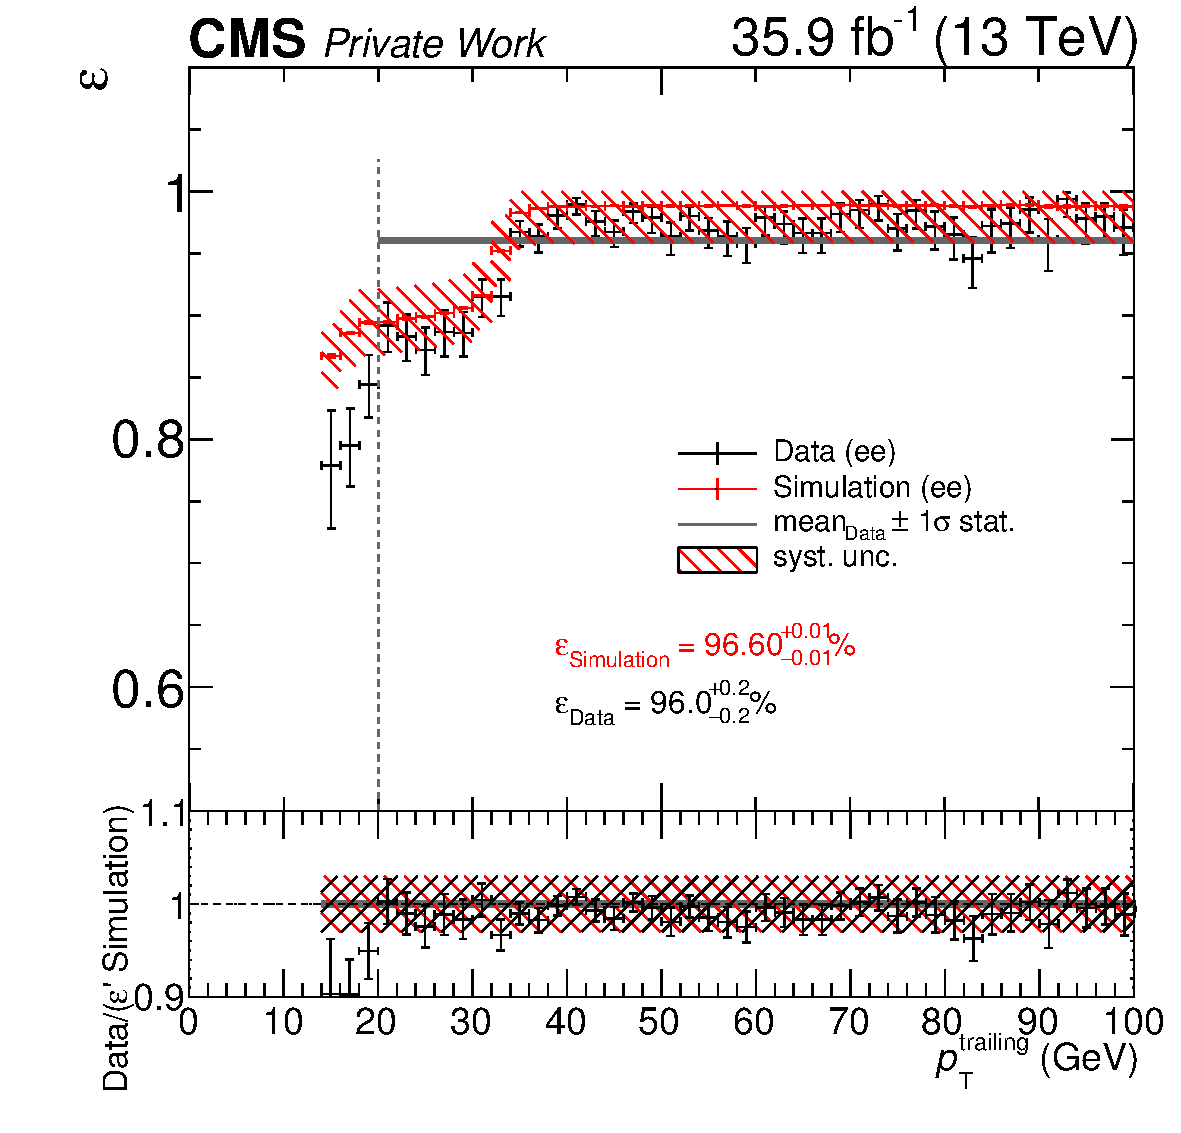
\includegraphics[width=\pairwidth]{figures/triggerStudies/efficiency_dataHT_trigDilep_EE_pt2}
 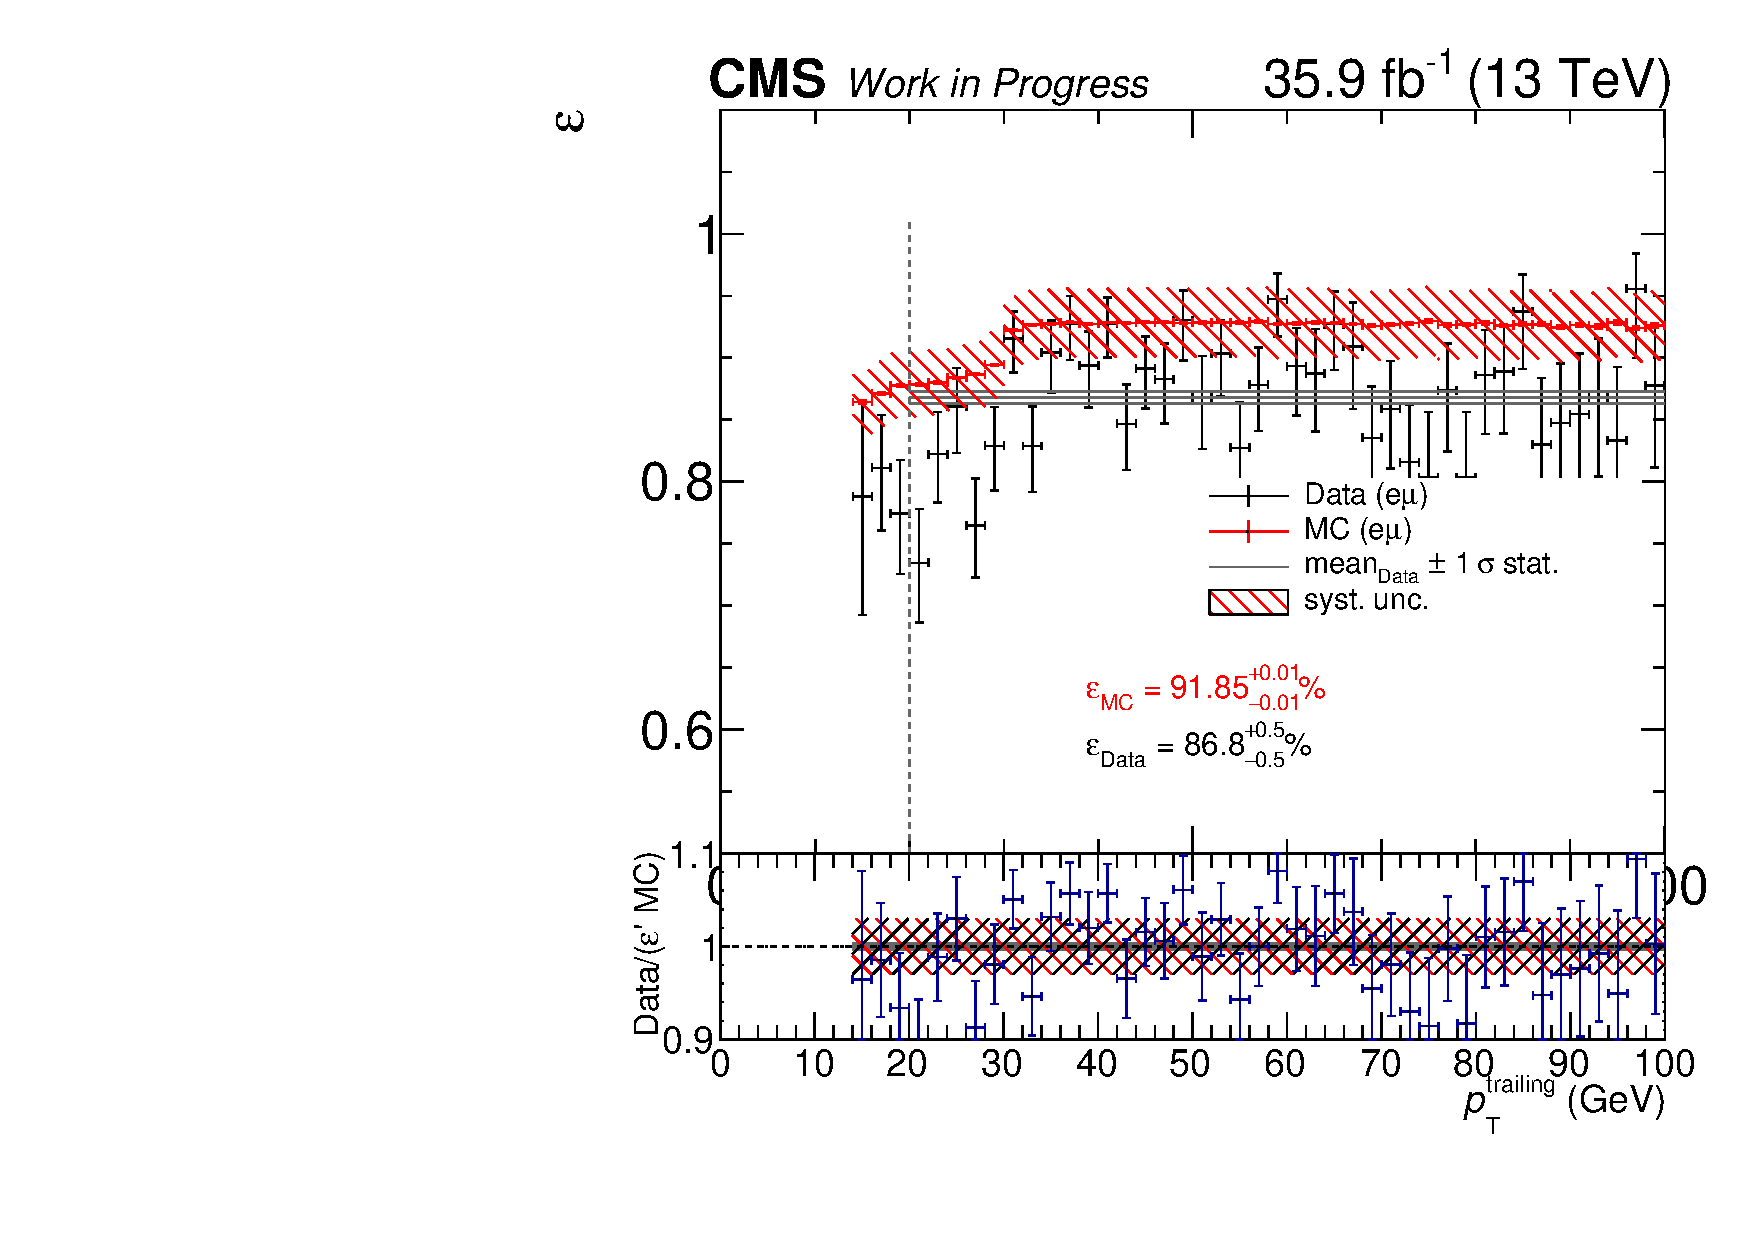
\includegraphics[width=\pairwidth]{figures/triggerStudies/efficiency_dataHT_trigDilep_EM_pt2}
 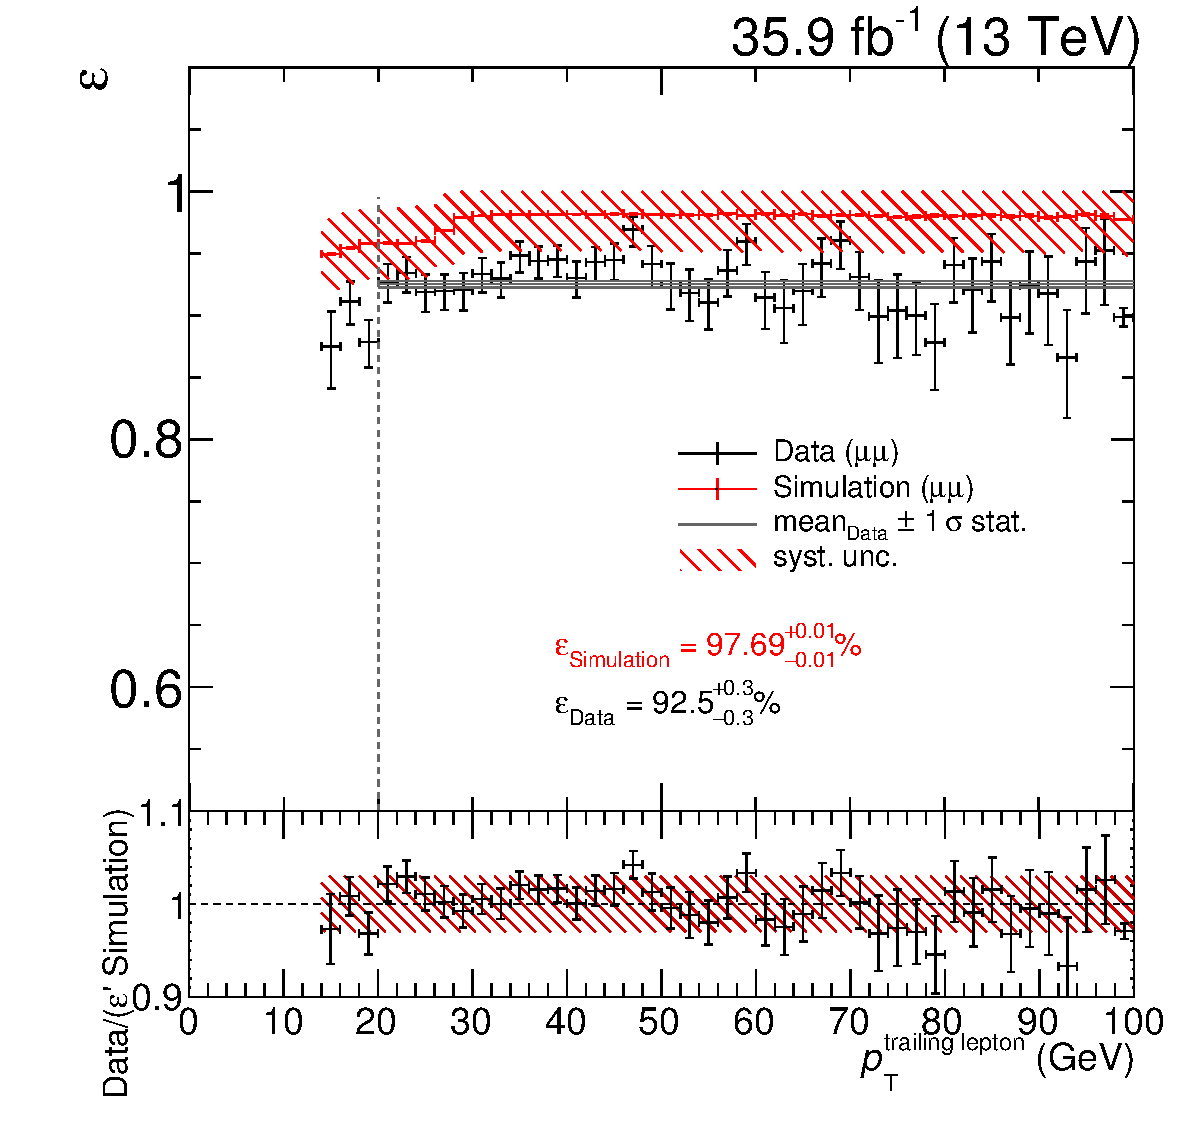
\includegraphics[width=\pairwidth]{figures/triggerStudies/efficiency_dataHT_trigDilep_MM_pt2}
 \caption{Measurement of the combined efficiency for all dilepton trigger combinations on data(black) and simulation(red) for the $\Pe\Pe$ (top left), $\Pe\PGm$ (top right), and $\PGm\PGm$ (bottom) channels. The measurement is performed using various $\HT$ baseline triggers, while the selection consists of the lepton pair preselection, and a $\HT>200\GeV$ requirement. The mean of the data efficiency with its statistical uncertainty (gray band), and the $3\%$ systematic uncertainty on the measurement (red band) are also shown.}
 \label{fig:triggEff}
\end{figure}


\begin{table}[htb]
 \centering
 \caption{Trigger efficiencies determined both on data and simulation for both baseline trigger
  configurations for the $\Pe\Pe$, $\Pe\Pgm$ and $\Pgm\Pgm$ channels.}
 \label{tab:triggEff}
 \begin{tabular}{lllll}
                   & \multicolumn{2}{c}{Data} & \multicolumn{2}{c}{Simulation}                                                         \\\hline
  baseline trigger & $\HT$                    & $\ptmiss$                      & $\HT$                     & $\ptmiss$                 \\\hline
  $\Pe\Pe$         & $96.0^{+0.2}_{-0.2}\%$   & $93.7^{+0.3}_{-0.3}\%$         & $96.60^{+0.01}_{-0.01}\%$ & $96.79^{+0.02}_{-0.02}\%$ \\
  $\Pe\Pgm$        & $86.6^{+0.5}_{-0.5}\%$   & $86.7^{+0.3}_{-0.3}\%$         & $91.85^{+0.01}_{-0.01}\%$ & $91.34^{+0.05}_{-0.05}\%$ \\
  $\Pgm\Pgm$       & $92.5^{+0.3}_{-0.3}\%$   & $93.9^{+0.3}_{-0.3}\%$         & $91.85^{+0.01}_{-0.01}\%$ & $97.62^{+0.02}_{-0.02}\%$ \\\hline
 \end{tabular}
\end{table}


In addition the agreement between rescaled simulation by the factor $\varepsilon'=\varepsilon_{Data}/\varepsilon_{MC}$ and data is shown in the ratio plots beneath the efficiency curves. It can be concluded, that the efficiency measurement works fine for both data and simulation, and the efficiencies agree within the systematic uncertainties, which is determined to be $3\%$ to account for the differences between simulation and data. This is indicated with the red uncertainty band in the plots.\\
As an additional independent check, the whole trigger efficiency measurement was performed on $\ptmiss$ datasets with $\ptmiss$ baseline triggers with thresholds of $110-600\GeV$. This selected phasespace region should be more or less orthogonal the $\HT$ selection. And in addition it is much closer to the final signal region, since the signal region selection will contain a $\ptmiss$ threshold, see \refSec{sec:SRSelection}. As can be read from \refTab{tab:triggEff}, the values obtained from this method are also in agreement with the efficiencies measured using the $\HT$ selection.
